\documentclass{article}
\usepackage{arxiv}
\usepackage[citations,hybrid,pipeTables,tableCaptions,underscores=false,codeSpans=false]{markdown}
\graphicspath{ {figures/} }

\title{An Instance-Based Account of Context Maintenance and Retrieval}


\author{
  Jordan B. Gunn \\
  Cognition and Cognitive Neuroscience Program \\
  Vanderbilt University \\
  Nashville, TN 37235 \\
  \texttt{jordan.gunn@vanderbilt.edu} \\
  \AND
  Sean M. Polyn \\
  Department of Psychological Sciences\\
  Vanderbilt University\\
  Nashville, TN 37235 \\
  \texttt{sean.polyn@vanderbilt.edu} \\
}

\begin{document}
\maketitle

\begin{abstract}
\markdownInput{../01_Abstract.md}
\end{abstract}

\keywords{Computational modeling \and episodic memory \and spacing effect}

\markdownInput{../02_Introduction.md}

%%\section{High-Level Approach}
%%\markdownInput{../03_Highlevel_Analysis.md}

\markdownInput{../04_Classic_CMR.md}

\markdownInput{../05_InstanceCMR.md}

\markdownInput{../06_Methods.md}

\section{Simulation of \citet{murdock1970interresponse}}
\markdownInput{../07_Baseline_Comparison.md}

\begin{figure}[h]
  \centering
  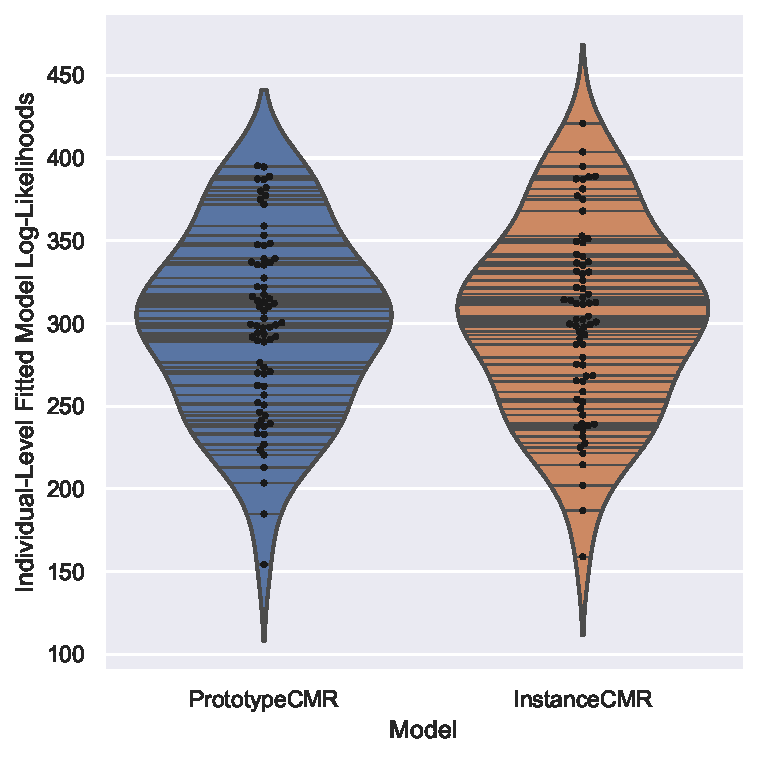
\includegraphics[width=.5\textwidth]{individual_murdock1970.pdf}
  \caption{Maximum log-likelihood of recall sequences exhibited by each subject \citep{murdock1970interresponse} under each considered model.}
  \label{fig:MurdOkaFits}
\end{figure}

\begin{figure}[h]
  \centering
  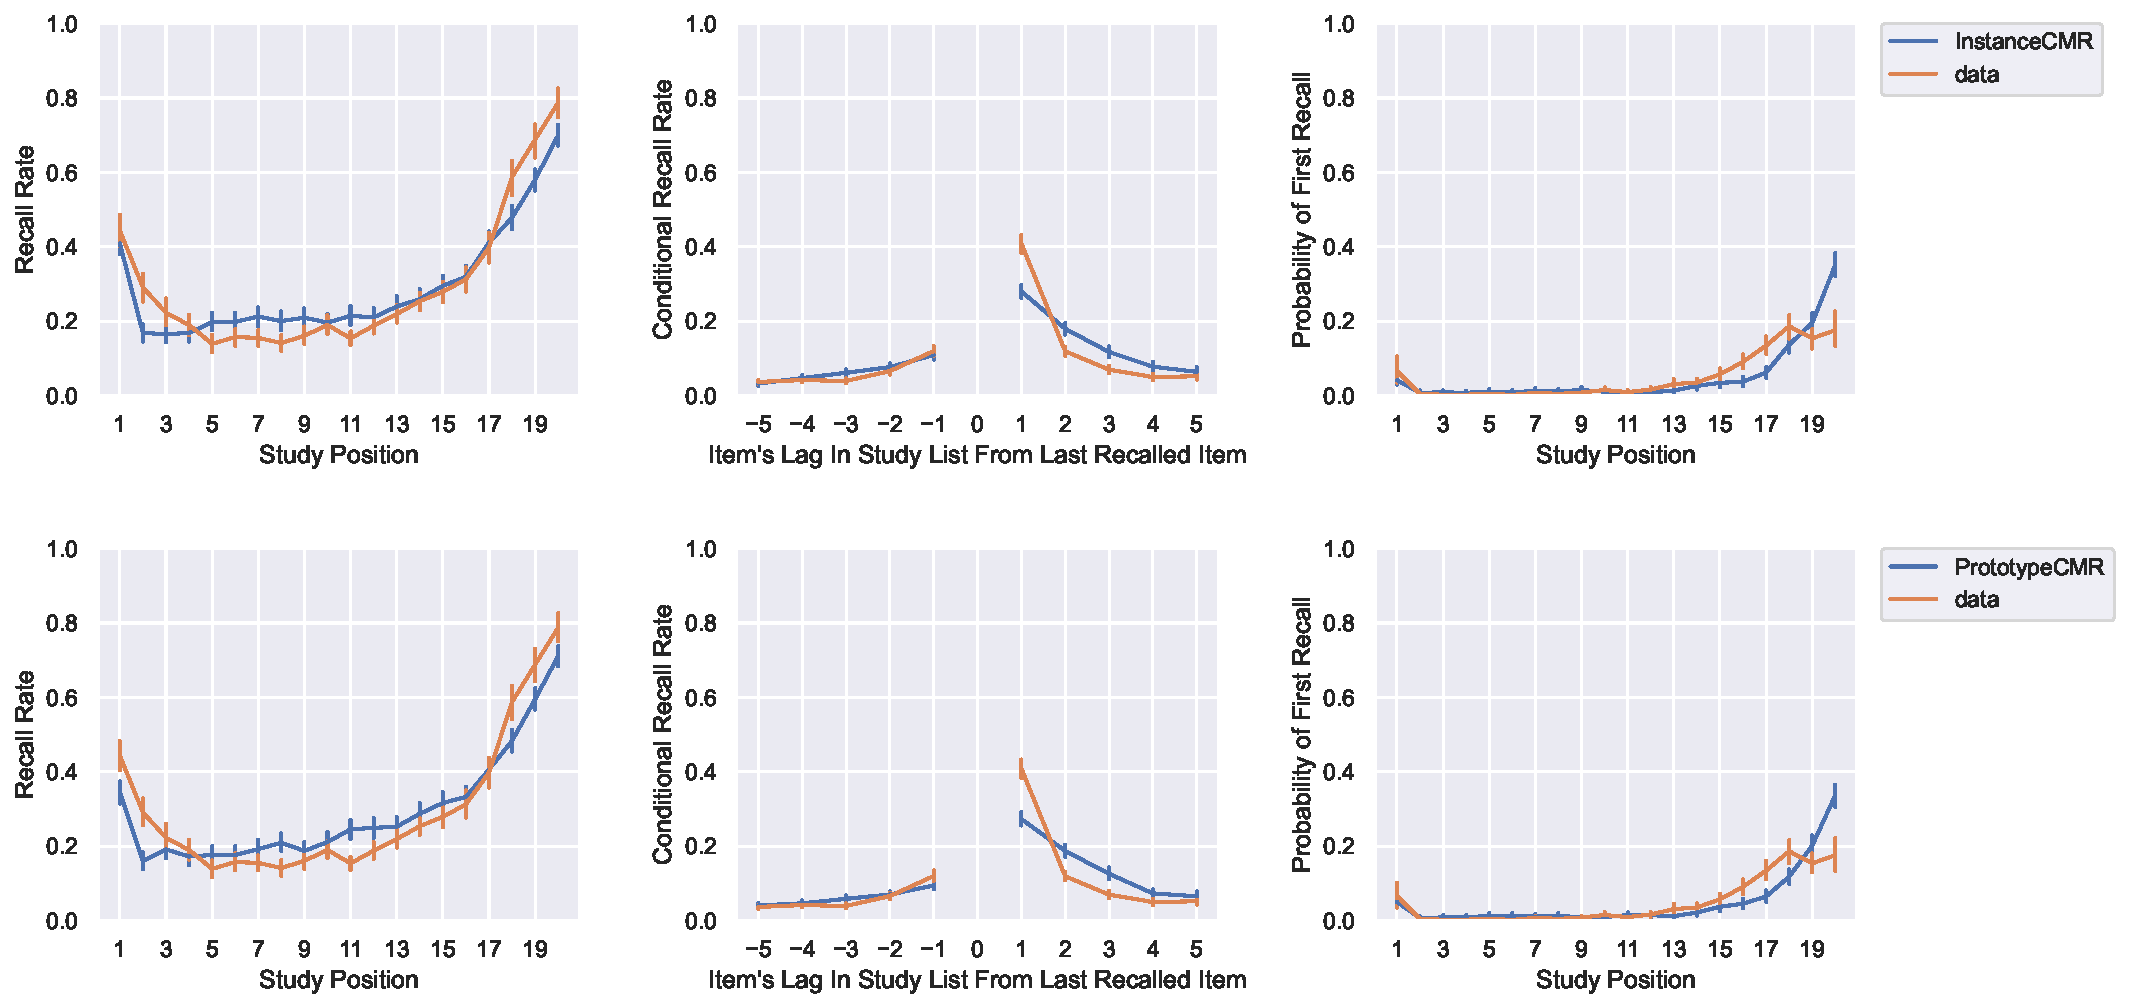
\includegraphics[width=.9\textwidth]{overall_murdock1970.pdf}
  \caption{Comparison of summary statistics between each model against observed data \citep{murdock1970interresponse}}
  \label{fig:MurdOkaSummary}
\end{figure}

\section{Simulation of \citet{murdock1962serial}}
\markdownInput{../08_Variable_List_Lengths.md}

\begin{figure}[h]
  \centering
  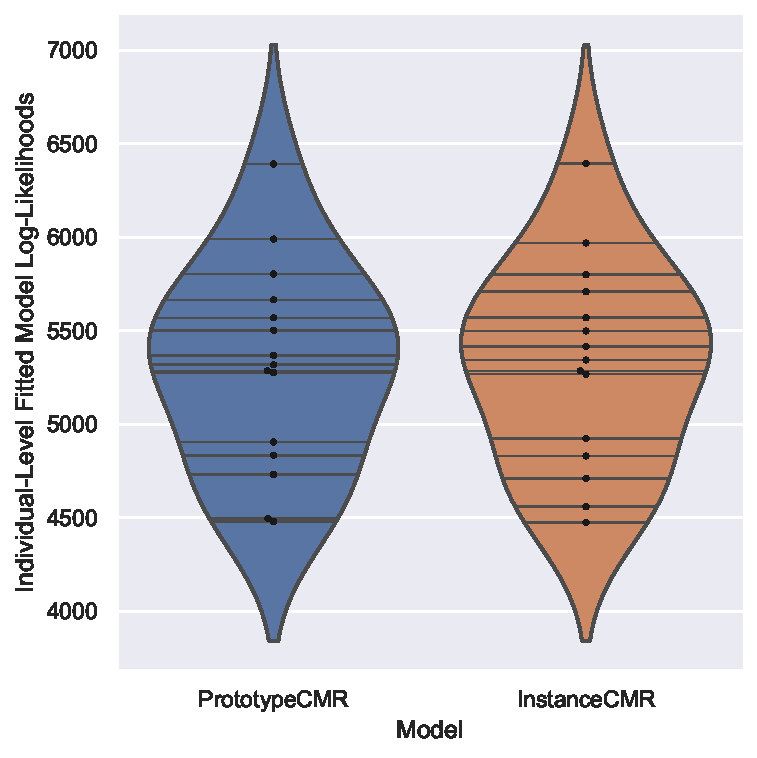
\includegraphics[width=.5\textwidth]{individual_murdock1962.pdf}
  \caption{Maximum log-likelihood of recall sequences exhibited by each subject under each considered model across list-lengths \citep{murdock1962serial}}.
  \label{fig:Murd62Fits}
\end{figure}

\begin{figure}[h]
  \centering
  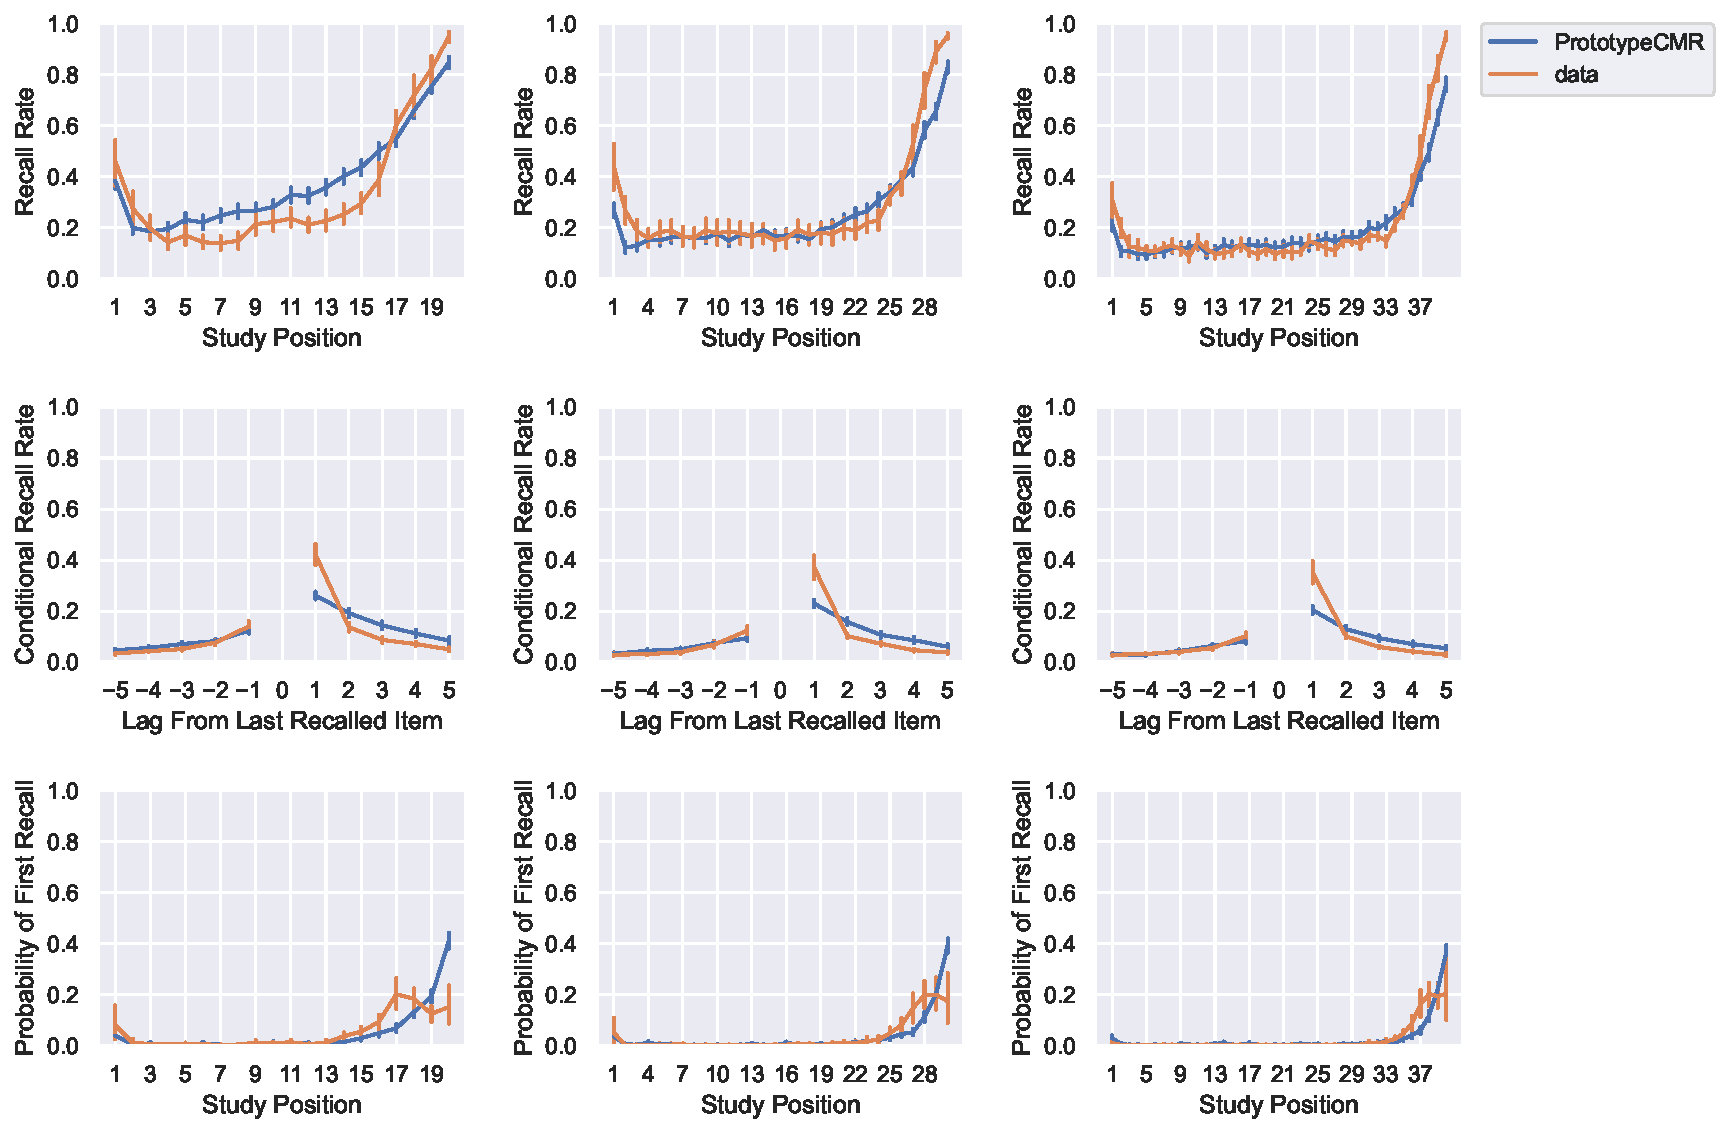
\includegraphics[width=.9\textwidth]{cmr_summary_murdock1962.pdf}
  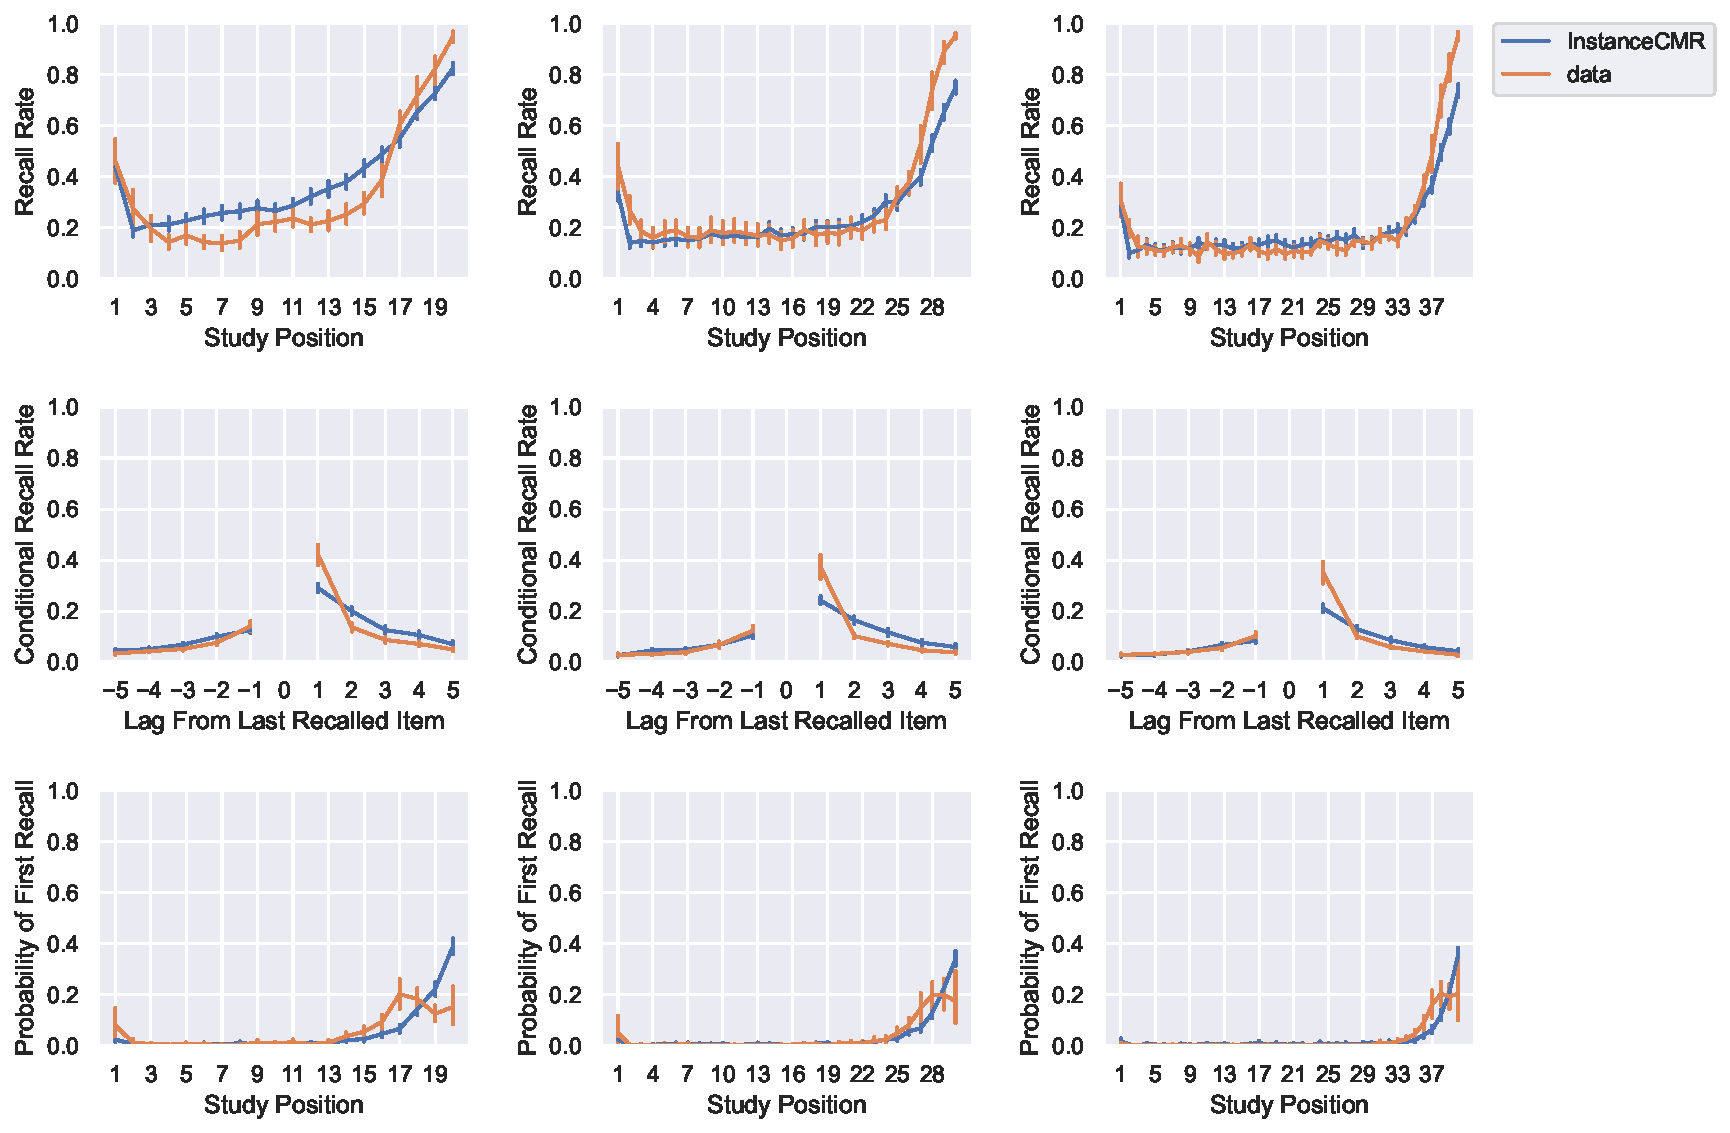
\includegraphics[width=.9\textwidth]{icmr_summary_murdock1962.pdf}
  \caption{Comparison of summary statistics between each model against observed data \citep{murdock1962serial}}.
  \label{fig:Murd62Summary}
\end{figure}


\section{Repetition Effects}
\markdownInput{../09_Item_Repetitions_Sims.md}

\begin{figure}[h]
  \centering
  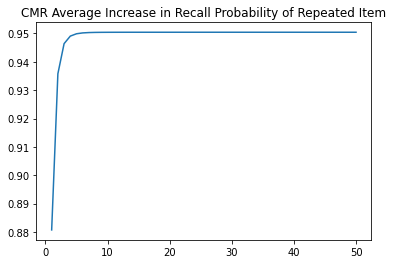
\includegraphics[width=.4\textwidth]{cmr_repeffect.png} 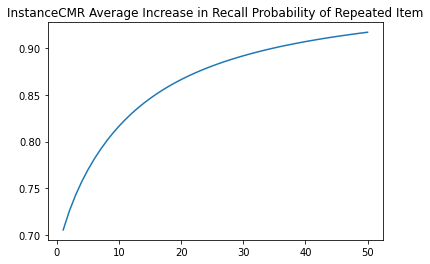
\includegraphics[width=.4\textwidth]{icmr_repeffect.png}
  \caption{Simulated effect of successive item repetitions on recall probability, by model, using parameters fitted over \citet{murdock1970interresponse} dataset.}
  \label{fig:repeffect}
\end{figure}

\markdownInput{../09_Item_Repetitions_Lohnas.md}

\begin{figure}[h]
  \centering
  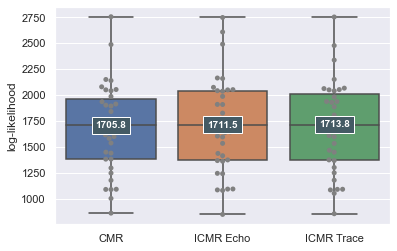
\includegraphics[width=.5\textwidth]{Lohnas_fit_all.png}
  \caption{Maximum log-likelihood of recall sequences exhibited by each subject under each considered model \citep{siegel2014retrieved}}
  \label{fig:LohnasFits}
\end{figure}

\begin{figure}[h]
  \centering
  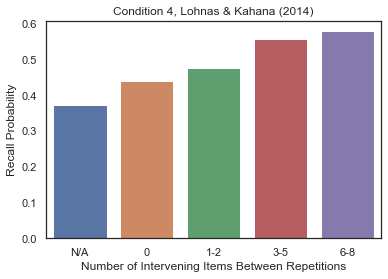
\includegraphics[width=.33\textwidth]{data_spacing.png} 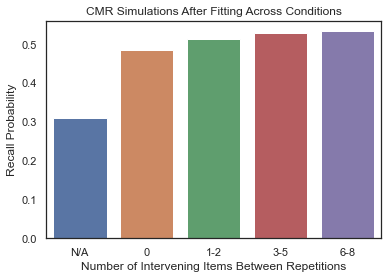
\includegraphics[width=.33\textwidth]{cmr_spacing.png} 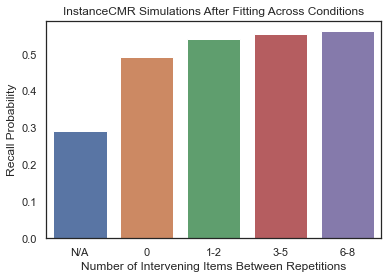
\includegraphics[width=.33\textwidth]{icmr_spacing.png}
  \caption{Recall probability as a function of spacing between item repetitions, if applicable.}
  \label{fig:LohnasSpacings}
\end{figure}

\section{Discussion}
\markdownInput{../10_Discussion.md}

\bibliographystyle{apalike}
\bibliography{../references}

\end{document}